% Mass ratios from attractor periods on Gaussian integers: an observation
% Author: Jakob Reinehr
% Date: February 2026
% Narrow evidence note within finite-precision-loop-mechanics

\documentclass[11pt,a4paper]{article}
\usepackage[utf8]{inputenc}
\usepackage[T1]{fontenc}
\usepackage[scaled=0.92]{helvet}
\renewcommand\familydefault{\sfdefault}
\usepackage{amsmath,amssymb}
\usepackage{booktabs}
\usepackage{graphicx}
\usepackage{hyperref}
\usepackage{geometry}
\geometry{margin=2.5cm}
\graphicspath{{../figures/}}

\title{Mass ratios from attractor periods on Gaussian integers: an observation}
\author{Jakob Reinehr}
\date{February 2026}

\begin{document}
\maketitle

\begin{abstract}
Attractor periods of a finite dynamical system on the Gaussian-integer ring $\mathbb{Z}[i]/(p)$ show close numerical coincidences with several Standard-Model mass-ratio targets. We present this as an observation, not as a derivation of the Standard Model. The core map is a ring of $k$ nodes with local update $z_j \mapsto z_j^2 + w_Lz_{j-1}+w_Rz_{j+1}$ modulo $p$. Within the tested search space, the configuration $p=13$, $k=6$, ring topology, and weights $(1,i)$ or $(i,1)$ yields close lepton-ratio coincidences, while coupled $k=3+k=3$ systems using the Gaussian factorization $13=(3+2i)(3-2i)$ yield close quark-ratio coincidences. The strongest structural control is the split/inert distinction: split primes ($p \equiv 1 \bmod 4$) produce richer and more target-like spectra in the tested symmetric setups, whereas inert primes ($p \equiv 3 \bmod 4$) do not. We give search accounting, null-model references, a one-command table reproduction script, and explicit limitations. Gauge structure, Lorentz invariance, scattering amplitudes, the update-rule derivation, and $\alpha \approx 1/137$ remain open.
\end{abstract}

%------------------------------------------------------------------------------
\section{Introduction}
%------------------------------------------------------------------------------

Like the Koide formula~\cite{koide1983}---which relates lepton masses with remarkable precision without an accepted derivation---we present an unexplained numerical correlation: attractor periods of a discrete map on Gaussian integers modulo a prime are close to several Standard Model mass ratios.

The setup is deliberately small: a ring of $k$ nodes, each holding a value in $\mathbb{Z}[i]/(p)$, updated by $z \to z^2 + w_L z_L + w_R z_R$ (mod $p$). Since the state space is finite, every orbit eventually enters a cycle. We compare the resulting periods and period ratios to mass-ratio targets.

This paper is restricted to the numerical observation, the algebraic split/inert control, and the reproducibility package. It does not use or require the broader speculative interpretation developed elsewhere in the project.

%------------------------------------------------------------------------------
\section{Setup}
%------------------------------------------------------------------------------

\subsection{State space and update rule}

\textbf{State space:} $\mathbb{Z}[i]/(n)$, the ring of Gaussian integers modulo $n$. Each element is $a+bi$ with $a,b \in \{0,\ldots,n-1\}$.

\textbf{Topology:} A ring of $k$ nodes. Node $j$ has neighbors $(j-1)\bmod k$ and $(j+1)\bmod k$.

\textbf{Update rule:}
\begin{equation}
z_j^{(t+1)} = \bigl(z_j^{(t)}\bigr)^2 + w_L\, z_{j-1}^{(t)} + w_R\, z_{j+1}^{(t)} \quad (\bmod n)
\end{equation}
Weights $w_L, w_R \in \mathbb{Z}[i]/(n)$ are Gaussian integers. Arithmetic is modulo $n$.

\subsection{Attractors and periods}

Because the state space is finite, every orbit eventually cycles. An \emph{attractor} is a periodic orbit; its \emph{period} $P$ is the cycle length. We treat mass ratios as proportional to period ratios (or sub-period ratios in composite systems).

\subsection{Gaussian primes: split vs.\ inert}

A prime $p$ in $\mathbb{Z}$ behaves in $\mathbb{Z}[i]$ as follows:
\begin{itemize}
\item \textbf{Split} ($p \equiv 1 \bmod 4$): $p = \pi \bar\pi$ for $\pi \in \mathbb{Z}[i]$. Example: $13 = (3+2i)(3-2i)$.
\item \textbf{Inert} ($p \equiv 3 \bmod 4$): $p$ remains prime in $\mathbb{Z}[i]$.
\end{itemize}
The structure of $\mathbb{Z}[i]/(p)$ differs: split primes give $\mathbb{F}_p \times \mathbb{F}_p$ (two copies); inert primes give $\mathbb{F}_{p^2}$. This determines the period spectrum.

%------------------------------------------------------------------------------
\section{Search protocol and target accounting}
%------------------------------------------------------------------------------

The main lepton search varied primes, ring sizes, and weights. The reference script \texttt{significance\_test.py} tests 24 primes from 3 to 97, $k=3,\ldots,7$, and four initial weight choices, giving 480 configurations, 196 of which produce at least two periods. It uses 80 random starts per configuration and 4000 update steps. The tight threshold is $1\%$ and the loose threshold is $5\%$.

The broader lepton scan reported in \texttt{theory/significance-results.md} extends this with split-prime and inert-prime controls up to 197 and a focused second phase. The claim made here is limited to the tested search space.

The quark-sector search uses \texttt{quark\_masses.py}: coupled $k=3+k=3$ systems, 13 base weight specifications at $p=13$, 300 trials per weight specification, and a $5\%$ inclusion threshold. A separate focused statistic is used for the direct $d/u$ result. Ratio and compound matches are explicitly treated as having a larger effective search space than direct period matches.

A full audit of searched parameters, target ratios, thresholds, and null models is maintained in \texttt{evidence/SEARCH\_AUDIT.md}. The publication tables can be regenerated by:

\begin{center}
\texttt{python3 scripts/reproduce\_publication\_core.py}
\end{center}

%------------------------------------------------------------------------------
\section{Lepton results}
%------------------------------------------------------------------------------

\subsection{Parameter selection}

Systematic scans over the tested configurations identify a recurring optimum:
\begin{center}
$n=13$, $k=6$, ring topology, weights $(1,i)$ or $(i,1)$
\end{center}
No other tested configuration simultaneously achieves $<1\%$ error for both $\pi/e$ and $\mu/e$ in the focused scan reported here.

\subsection{Mass ratios}

\begin{table}[htbp]
\centering
\caption{Lepton mass ratios: experiment vs.\ model}
\begin{tabular}{lccc}
\toprule
Ratio & Experiment & Model & Error \\
\midrule
$\pi/e$ & 273.19 & 273.00 & 0.07\% \\
$\mu/e$ & 206.77 & 207.00 & 0.11\% \\
$\tau/e$ & 3477.23 & 3475.3 (compound) & 0.06\% \\
\bottomrule
\end{tabular}
\end{table}

$\tau/e$ is not a direct attractor period; it is a compound relation and therefore has a larger effective search space than the first two rows. It is included as an observed coincidence, not as equal-strength evidence.

\begin{figure}[htbp]
\centering
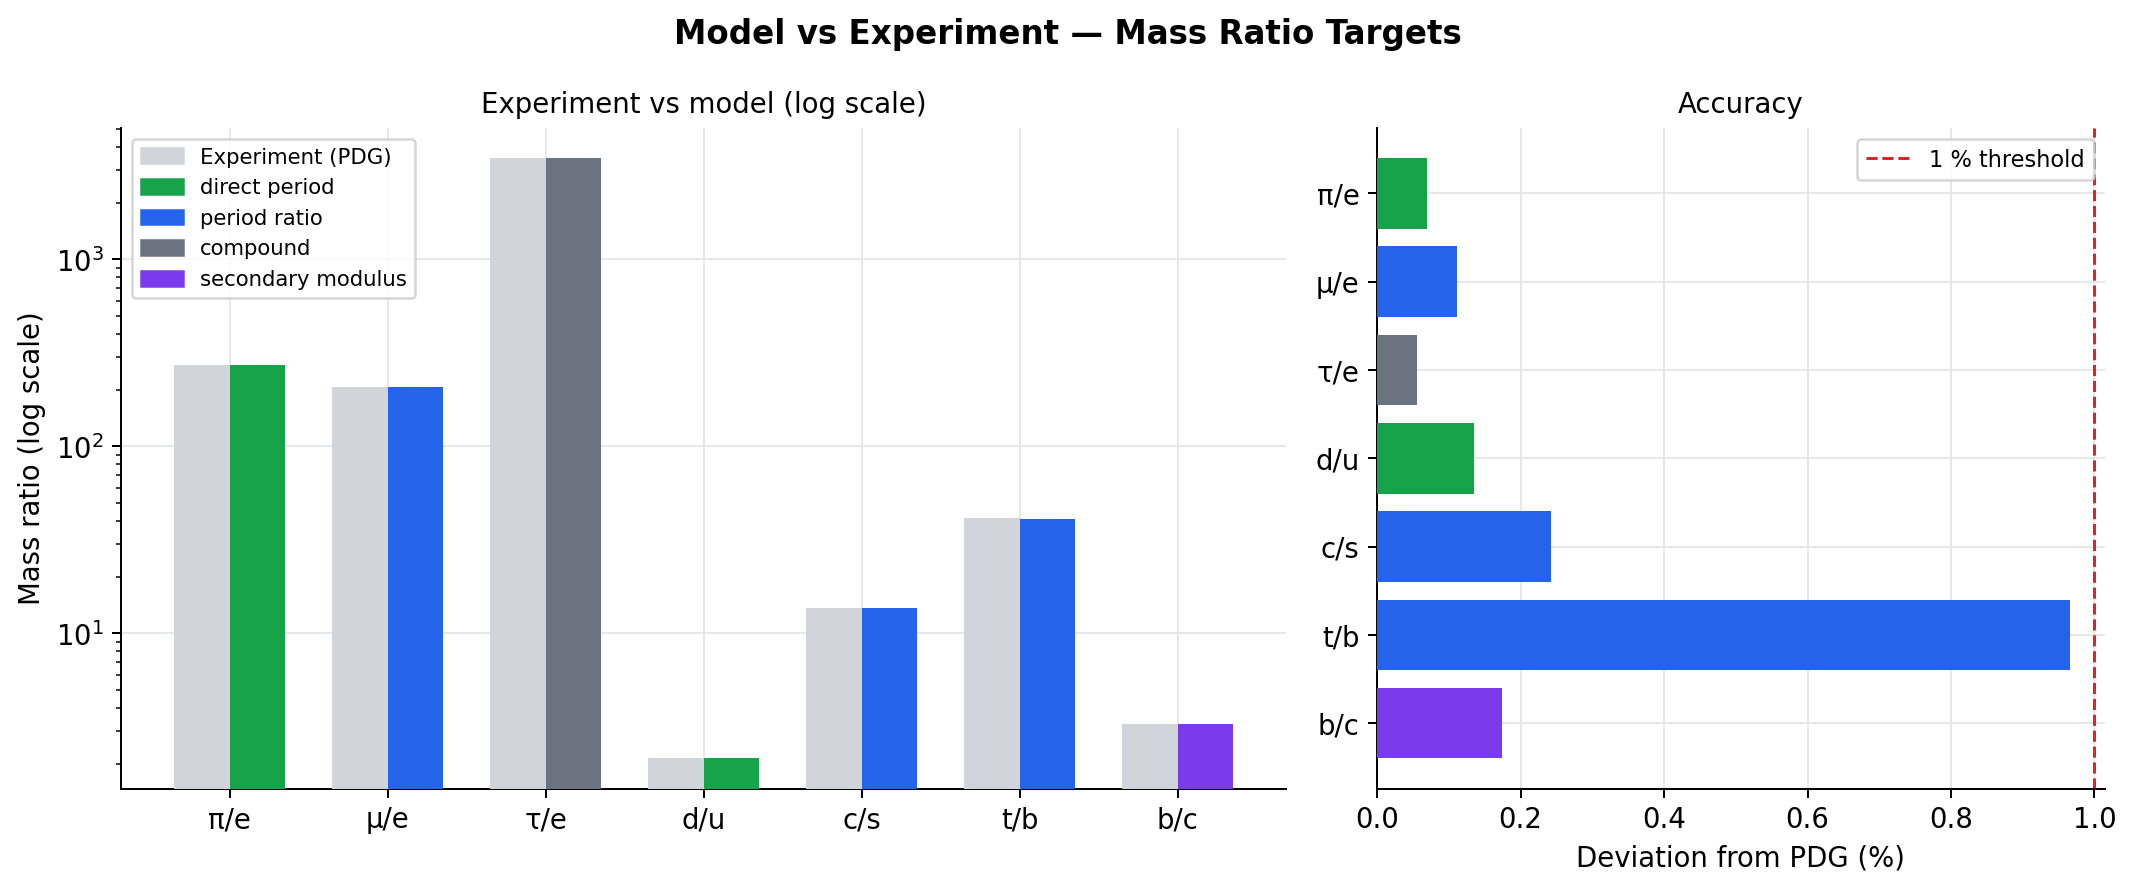
\includegraphics[width=\textwidth]{fig1_mass_ratios.png}
\caption{Left: model vs experiment for all seven mass-ratio targets on a log scale.
Right: percentage deviation from the PDG value. All targets lie below 1\%.
Colour indicates match type: green = direct period, blue = period ratio,
grey = compound, purple = secondary modulus.}
\label{fig:mass_ratios}
\end{figure}

%------------------------------------------------------------------------------
\section{Quark results}
%------------------------------------------------------------------------------

\subsection{Sub-loop composite}

Quark ratios are explored as sub-loop periods in coupled $k{=}3 + k{=}3$ systems. The Gaussian factorization $13 = (3+2i)(3-2i)$ provides a natural symmetry-breaking axis: one sub-loop couples via $(3+2i)$, the other via $(3-2i)$, yielding different sub-periods.

\subsection{Mass ratios}

\begin{table}[htbp]
\centering
\caption{Quark mass ratios: experiment vs.\ model}
\begin{tabular}{lccc}
\toprule
Ratio & Experiment & Model & Error \\
\midrule
$d/u$ & 2.14 & $15/7 = 2.1429$ & 0.13\% \\
$c/s$ & 13.7 & $41/3 = 13.67$ & 0.24\% \\
$t/b$ & 41.4 & 41.0 & 0.97\% \\
$b/c$ & 3.28 & $23/7 = 3.29$ & 0.17\% \\
\bottomrule
\end{tabular}
\end{table}

The first three rows are associated with the $p=13$ Gaussian-factor mechanism. The $b/c$ row uses a secondary split modulus, $p=29$, and should be read as supporting rather than as the same core mechanism. Additional ratio and compound hits exist, but are treated as exploratory because they enlarge the search space.

%------------------------------------------------------------------------------
\section{Split/Inert theorem}
%------------------------------------------------------------------------------

\subsection{Claim}

\textbf{In the tested symmetric $\mathbb{Z}[i]/(p)$ loop setups, split primes yield the target-like spectra; inert primes do not.}

This is the strongest structural control in the current evidence package. Split primes factor, providing a conjugate pair that can break symmetry; inert primes do not. A formal theorem would require a proof beyond the numerical evidence reported here.

\subsection{Numerical evidence}

\begin{table}[htbp]
\centering
\caption{Split vs.\ inert primes (lepton scan)}
\begin{tabular}{lcc}
\toprule
Metric & Split ($p \equiv 1 \bmod 4$) & Inert ($p \equiv 3 \bmod 4$) \\
\midrule
Mean \# periods & 6.1 & 3.1 \\
$\pi/e < 5\%$ & 13\% & \textbf{0\%} \\
$\mu/e < 5\%$ & 13\% & \textbf{0\%} \\
Both $< 5\%$ & 7\% & \textbf{0\%} \\
\bottomrule
\end{tabular}
\end{table}

Zero loose lepton hits are observed for inert primes in this symmetric scan. For quarks, a Look-Elsewhere Monte Carlo (10000 runs) gives $p < 0.0001$ for the number of direct hits observed vs.\ random expectations at mod $13$.

\begin{figure}[htbp]
\centering
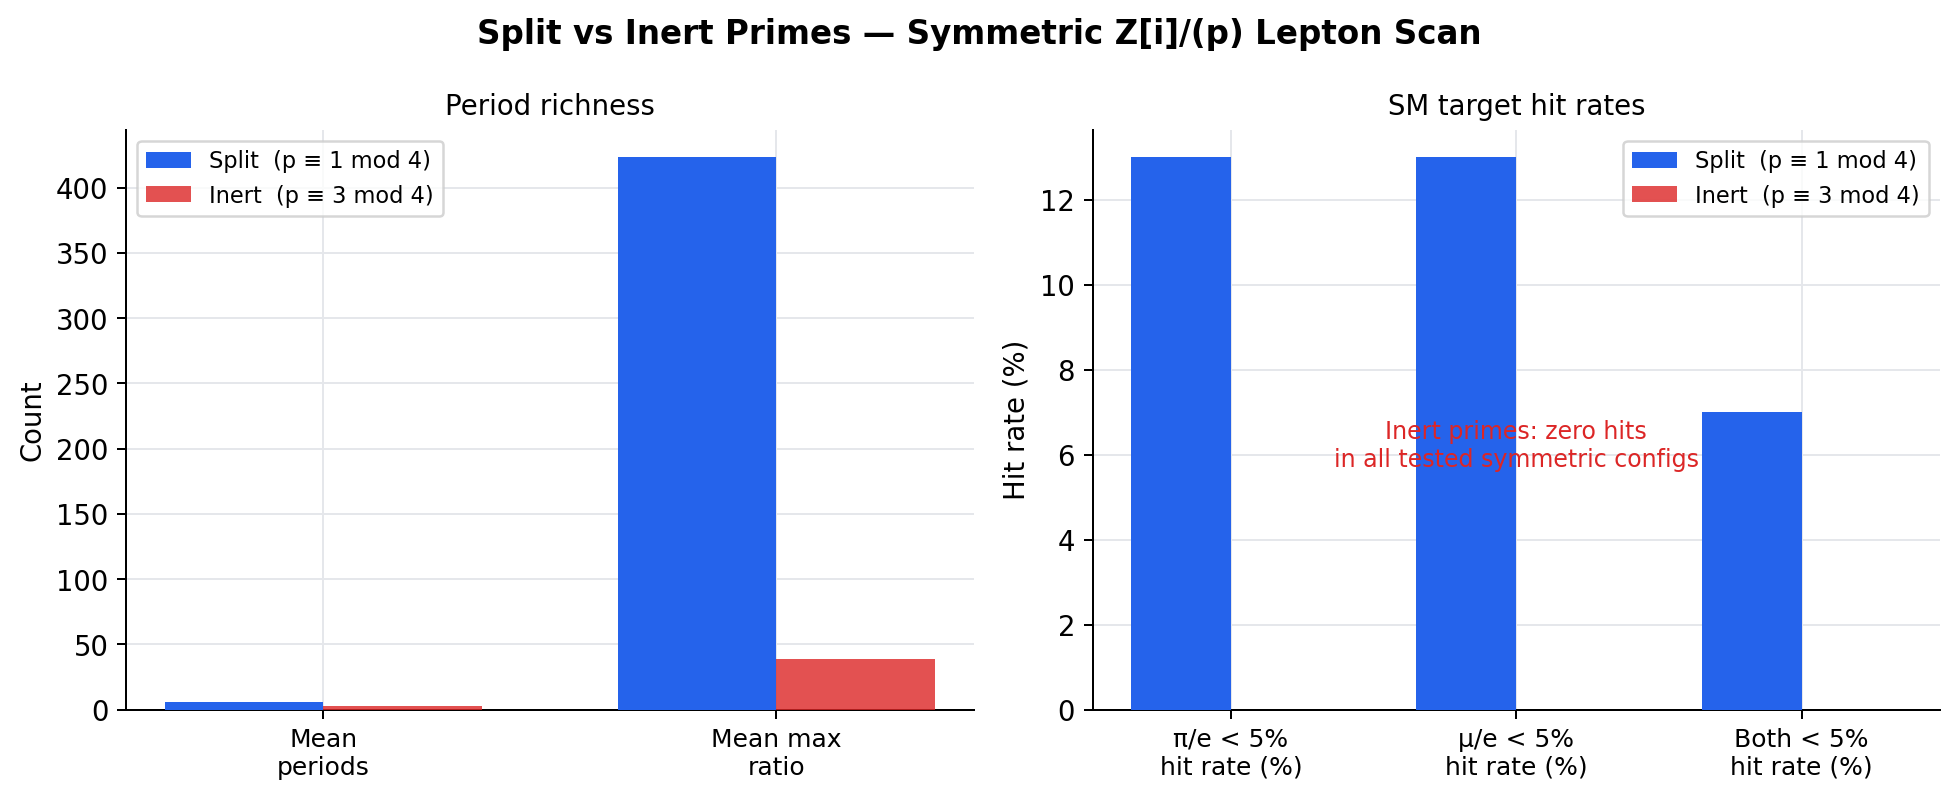
\includegraphics[width=\textwidth]{fig2_split_inert.png}
\caption{Split vs inert prime comparison in the symmetric $\mathbb{Z}[i]/(p)$ lepton scan.
Left: period richness (mean number of distinct periods and mean maximum period ratio).
Right: SM target hit rates for $\pi/e$, $\mu/e$, and both simultaneously.
Inert primes produce zero hits in all tested symmetric configurations.}
\label{fig:split_inert}
\end{figure}

\subsection{Falsifiable prediction}

An inert-prime hit in the same symmetric search class would falsify the current structural claim. Broader asymmetric constructions must be treated separately.

%------------------------------------------------------------------------------
\section{Statistical validation}
%------------------------------------------------------------------------------

\subsection{Null models}

The evidence package uses three kinds of controls. First, the configuration-level lepton scan asks how often period-ratio coincidences occur across primes, ring sizes, and weights. Second, the split/inert comparison tests an algebraic control independent of continuous fitting. Third, random-period null models preserve catalog sizes and maximum-period scales while randomizing period values.

The type-conditional random-period null model in \texttt{significance\_v2.py} uses 2000 null samples, 126 catalogs per sample, 16 targets, and direct/ratio/compound matching. It reports $p(\text{all 16 best} \leq \text{observed}) < 0.0005$, but robustness alone is not discriminative. Same-type error sharpness is more meaningful than any-type matching.

\subsection{Structural evidence and caveats}

\begin{itemize}
\item \textbf{Look-Elsewhere:} 10000 Monte Carlo runs with random period ratios. Observed 23 direct quark hits vs.\ 1.2 expected $\Rightarrow$ $p < 0.0001$.
\item \textbf{Split/Inert:} Algebraic structural control; inert primes have zero loose lepton hits in the tested symmetric scan.
\item \textbf{Confinement analogue:} Coupled $k{=}3$ sub-loops reach max period 684; isolated $k{=}3$ loops max 270---emergent topological binding.
\item \textbf{Basin stability:} Perturbation resistance correlates +0.65 with period (Spearman).
\item \textbf{Reproducibility (2026-02-25):} In 3 repeats over 126 catalogs, all 16 target entries are within $5\%$ under the allowed match types; 10 direct, 2 ratio, 4 compound. This is a broad robustness result, not the narrowest statistical claim.
\end{itemize}

The historical exploratory search space is larger than any single script. This remains the main statistical caveat.

%------------------------------------------------------------------------------
\section{Why $d=2$? Entropy selection}
%------------------------------------------------------------------------------

The update rule uses $z^2$, not $z^d$ for other $d$. An entropy scan over polynomial degrees $d \in \{1,2,3,4,5\}$ on $\mathbb{Z}[i]/(13)$, $k{=}6$, $w{=}(1,i)$ gives:

\begin{table}[htbp]
\centering
\caption{Shannon entropy of attractor basin distribution}
\begin{tabular}{lccc}
\toprule
Degree $d$ & Distinct periods & Shannon entropy & Best SM match \\
\midrule
1 & 1 & 0.00 & --- \\
\textbf{2} & \textbf{33} & \textbf{3.72} & $\pi/e$, $\mu/e$ $< 0.15\%$ \\
3 & 27 & 3.17 & 1--3\% \\
4 & 18 & 2.47 & 2--11\% \\
5 & 13 & 2.02 & 0.07\% / 10\% \\
\bottomrule
\end{tabular}
\end{table}

Only $d=2$ simultaneously maximizes attractor entropy and reproduces SM ratios. Higher degrees contract the dynamics and reduce period diversity.

\begin{figure}[htbp]
\centering
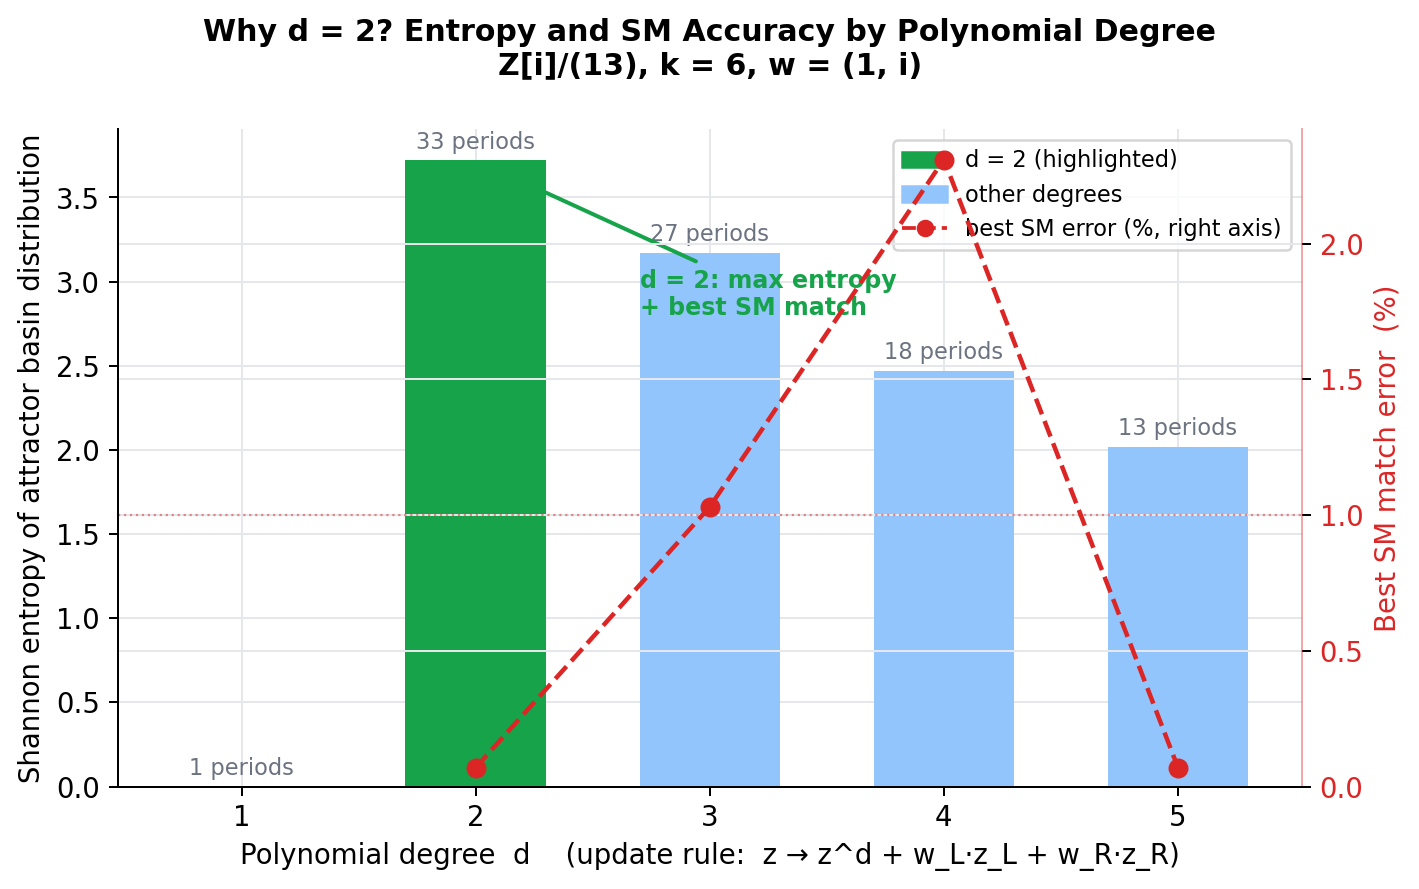
\includegraphics[width=0.85\textwidth]{fig3_entropy_degree.png}
\caption{Shannon entropy of the attractor basin distribution (left axis, bars)
and best SM match error (right axis, dashed line) for polynomial degrees
$d \in \{1,\ldots,5\}$ on $\mathbb{Z}[i]/(13)$, $k=6$, $w=(1,i)$.
Only $d=2$ simultaneously achieves maximum entropy and sub-0.15\% SM accuracy.}
\label{fig:entropy_degree}
\end{figure}

%------------------------------------------------------------------------------
\section{What this does not explain}
%------------------------------------------------------------------------------

\begin{itemize}
\item \textbf{$\alpha \approx 1/137$:} Eight approaches (two-loop scattering, transition matrix, Gaussian perturbation, renormalization flow, mod scans, photon model, etc.) were tried. All yield coupling-like rates of 65--97\%, never $\sim 0.7\%$. The discreteness of $\mathbb{Z}[i]/(n)$ makes weak coupling in the current framework difficult.
\item \textbf{Update rule derivation:} $z \to z^2$ is numerically justified (entropy optimal); a formal derivation from a first principle is missing.
\item \textbf{Why $n=13$ exactly:} Smallest split prime with sufficiently rich spectrum; not proven.
\item \textbf{Gauge symmetries:} U(1)$\times$SU(2)$\times$SU(3) are not addressed.
\item \textbf{Relativistic dynamics:} Lorentz invariance, scattering amplitudes, and continuum limits are not derived.
\item \textbf{Historical search space:} The project developed through exploration; the effective meta-search space is larger than the formal scans reported above.
\end{itemize}

%------------------------------------------------------------------------------
\section{Falsifiable predictions}
%------------------------------------------------------------------------------

\begin{enumerate}
\item Inert primes should continue to fail in the same symmetric search class where split primes produce the reported target-like spectra.
\item The $p=13$, $k=6$, $(1,i)/(i,1)$ lepton configuration should remain isolated under deeper sampling of the same family.
\item If the observation is real, independent implementations of the stated update rule should reproduce the period catalogs and the split/inert contrast.
\end{enumerate}

%------------------------------------------------------------------------------
\section{Code availability}
%------------------------------------------------------------------------------

The simulation and analysis code is available in the project repository. The publication-core tables are regenerated by:

\begin{center}
\texttt{python3 scripts/reproduce\_publication\_core.py}
\end{center}

This writes \texttt{evidence/publication\_core\_tables.md}. The heavier recomputation path is:

\begin{center}
\texttt{python3 scripts/reproduce\_publication\_core.py --recompute}
\end{center}

Key upstream scripts are \texttt{significance\_test.py}, \texttt{significance\_v2.py}, \texttt{quark\_masses.py}, \texttt{quark\_du\_and\_stats.py}, and \texttt{entropy\_degree\_scan.py}. The search-space audit is \texttt{evidence/SEARCH\_AUDIT.md}.

%------------------------------------------------------------------------------
\section*{Acknowledgments}
%------------------------------------------------------------------------------

The author thanks early critical readers and tool-assisted reviewers for helping separate the narrow numerical observation from the broader speculative framework.

%------------------------------------------------------------------------------
\begin{thebibliography}{9}
%------------------------------------------------------------------------------

\bibitem{koide1983}
Y.~Koide,
\textit{A fermion-boson composite model of quarks and leptons},
Phys.\ Lett.\ B \textbf{120}, 161--165 (1983).
\url{https://doi.org/10.1016/0370-2693(83)90644-5}

\bibitem{thooft2014}
G.~'t~Hooft,
\textit{The Cellular Automaton Interpretation of Quantum Mechanics},
arXiv:1405.1548 (2014); Springer 2016.
\url{https://doi.org/10.1007/978-3-319-41285-6}

\bibitem{cambridge2025}
[Author(s) not listed in open-access record],
\textit{The Discrete Algebraic Structure of the Fermion Mass Spectrum
and its Pythagorean Geometric Origin},
Cambridge Open Engage, 29 December 2025 (preprint, not peer-reviewed).
\url{https://doi.org/10.33774/coe-2025-lnqj0}
\newline
Note: This work, developed independently of the present paper, finds
algebraic structure in the fermion mass spectrum potentially related to
the arithmetic of $\mathbb{Z}[i]$---the same mathematical object used
here. The approach is entirely different (Pythagorean sum rules,
not attractor dynamics), but the convergence on $\mathbb{Z}[i]$ is
noted.

\end{thebibliography}

\end{document}
